% \chapter{Technical Fundamentals}
% Since the main part of this thesis addresses the implementation of flow control algorithms for a left ventricular assist device, the basics of control theory and a introduction on iterative learning control will be presented here as well.

\chapter{Control Theory}
Since the field of control theory is very extensive, this section will only deal with the notation and structure of a standard control loop in general. Furthermore, the basic principles of a PI controller and an iterative learning control are discussed, since these are used within pratical part of the thesis.
\section{Fundamentals}
The basic task of control engineering is to influence a time-varying process from the outside with the goal that the process is executed in a predetermined manner. A control system is characterized in particular by the feedback of the controlled variable to the reference variable. The reference variable represents the state to be achieved.
In theory, this is represented by a control loop with the components shown in \figurename~{\ref{fig:control_loop}}.
\begin{figure}
  \centering
  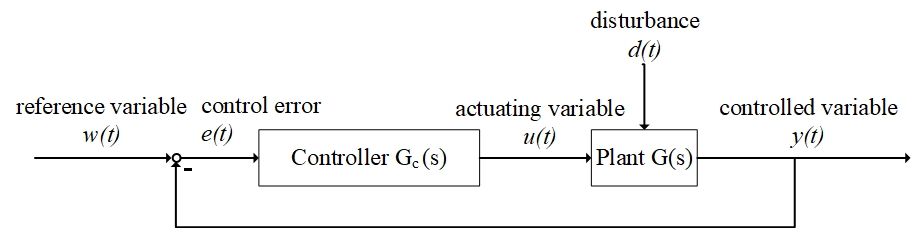
\includegraphics[width=0.9\textwidth]{images/control_loop.jpg}
  \caption[General structure of a control loop]{General structure of a control loop}
  \label{fig:control_loop}
\end{figure}
The plant $G(s)$ transfers the actuating variable $u(t)$, as well as the influence of the the disturbance $d(t)$, to the controlled variable $y(t)$. This variable is permanently compared with the reference variable $w(t)$ by means of a feedback. Which results in the control error
\begin{equation}
  e(t) = w(t) - y(t)
 \label{eq:e_t}
\end{equation}
The controller $G_{c}(s)$ then transfers the control error to the actuating variable again. The aim of the control loop is to achieve the smallest possible control error with the greatest possible damping. Since these goals contradict each other, a trade off must always be accepted here.\cite{Reg_17}
\\However, there are some general requirements for the closed control loop, which have to be fulfilled. The first of which states that the closed loop needs to be stable. This is the case when the control loop responds to a finite excitation with a finite output signal. The second one is the requirement for disturbance rejection, stating that the controlled variable needs to follow the reference variable asymptotically, so that
\begin{equation}
    \lim\limits_{t \rightarrow \infty}{e(t)} = 0
 \label{eq:lim_e}
\end{equation}
Another requirement is that the dynamic relationship between the reference variable w(t) and the controlled variable y(t) must satisfy specified quality requirements.  The last requirement states that the first three requirements must be statisfied despite uncertainties in the plant. This requirement is called the Robustness requirement. More detailed information on these requirements can be found in \cite{Reg_10}.

The plant $G(s)$ corresponds to the part of the system in which the physical quantity to be controlled is influenced by the controller. The calculation of the plant by setting up and solving differential equations is only possible in a few cases. Due to this, the determination of the plant's characteristic values is usually carried out experimentally. There are several basic types of plants. These are classified according to their dynamic behavior. As only the PT$_{1}$-element is used in the practical part of this thesis, all other variations will not be discussed at this point. Detailed information on this topic can be found in \cite{Reg_10}.
\\The PT$_{1}$-element is the plant type which is most common in technical equipment. A PT$_{n}$-element, in it's static state, reacts proportionally to the input value and has a distinct transition behavior. The index n describes the system order. A PT$_{1}$-element therefore is a proportional delay element of first order. The mathematical formulation of the transfer function of a PT$_{1}$-element is
\begin{equation}
    G(s) = \frac{k_{s}}{1+sT}
 \label{eq:tf_pt1}
\end{equation}

\begin{figure}[h]
   \centering
   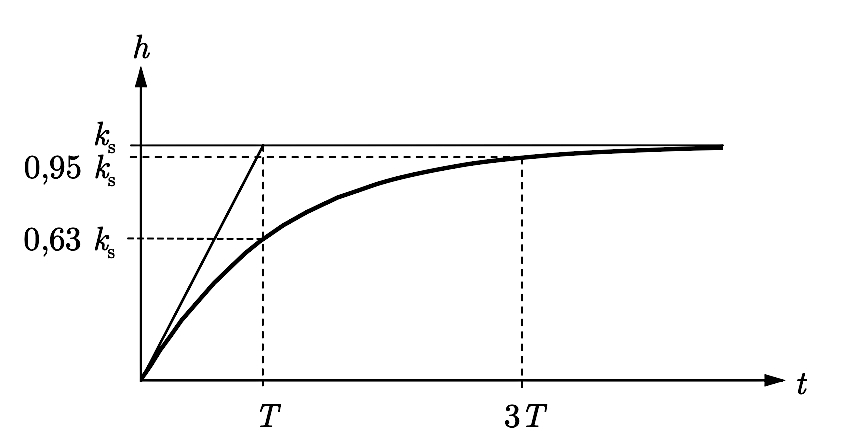
\includegraphics[width=0.9\textwidth]{images/tf_pt1.jpg}
   \caption[Tranfer function of a PT$_{1}$-element]{Transfer function of a PT$_{1}$-element \cite{Reg_10}.}
   \label{fig:tf_pt1}
 \end{figure}
The value $k_{s}$ describes the static gain, which equals the final value of the transfer function, in case $u(0)=0$. The time constant T enables an impression of the speed with which the system can react to changes at the input. It is defined as the time at which the transfer function reaches 63\% of the static gain. \cite{Reg_10}
\figurename~\ref{fig:tf_pt1} shows the tranfer function of a PT$_{1}$-element.


\section{PI-controller}
A PI-controller is a control structure commonly used for linear systems. This structure consists of both a propotional and an integral control element.
The output value of a P-controller is proportional to it's input value. In relation to the control loop in \figurename~\ref{fig:control_loop} this leads to
\begin{equation}
    u(t) = K_{P}e(t).
 \label{eq:p_contr_1}
\end{equation}
Using Laplacetransformation the transfer function for a P controller can be determined as
\begin{equation}
    G(s) = \frac{u(s)}{e(s)} = K_{P}
 \label{eq:p_contr_2}
\end{equation}
Therefore, the step response of this controller equals a step weighted with the Parameter $K_{P}$.
The relationship between input and output value of an I-controller is described through
\begin{equation}
    u(t) = K_{I}\int e(t) dt.
 \label{eq:i_contr_1}
\end{equation}
Equal to the P-controller, Laplacetransformation can be used to determine the transfer function of the I-controller.
This leads to
\begin{equation}
    G(s) = \frac{u(s)}{e(s)} = \frac{K_{I}}{s},
 \label{eq:i_contr_2}
\end{equation}
which indicates a step response in form of a ramp with slope $K_{I}$.
In order to generate a PI-controller from these elements the elements can be added, which leads to
\begin{equation}
    u(t) = K_{P}e(t) + K_{I}\int e(t) dt.
 \label{eq:pi_contr_1}
\end{equation}
The Laplacetransformation can be used again to formulate the transfer function
\begin{equation}
    G(s) = \frac{u(s)}{e(s)} =  K_{P} + \frac{K_{I}}{s}.
 \label{eq:pi_contr_2}
\end{equation}
The step response of the PI-controller, illustrated in \figurename~\ref{fig:step_resp_pi}, shows both the weigthed step from the P-controller and the ramp from the I-controller.

\begin{figure}[h]
   \centering
   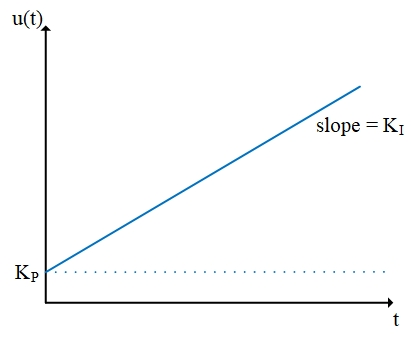
\includegraphics[width=0.4\textwidth]{images/step_resp_pi.jpg}
   \caption[Step response of a PI-Controller]{Step response of a PI-Controller}
   \label{fig:step_resp_pi}
 \end{figure}

\subsection{Tuning rules}
In regards to the controller parameters, tuning is of great importance. If the parameters are chosen incorrectly it can lead to poor performance. There are many different approach to tuning a PI-Controller in order to achieve the best system performance. These are reaching from heuristic methods, over analysis of pole-zero plots, to computer-aided numerical parameter optimization \cite{Reg_10} At this point only the tuning rules according to Ziegler Nichols (ZN) and the rules according to Chien Hrones Reswick (CHR) will be discussed, as these have been used for the implementation of flow control in the practical work.  Information on other approaches can be found in \cite{Reg_11}.

\subsubsection{Tuning rules according to Ziegler Nichols}
The tuning rules according to Ziegler Nichols are on of the most commoly used heuristic methods in tuning controller parameters for PID-Controllers. They are used especially, if a mathematical model of the plant is not available, but the plant can be approximated as a PT$_{n}$-element. \cite{Reg_17}
A necessary condition is that the step response of the plant needs to be experimentally identifiable without risk of damage to the system. After the step response has been determined, it is displayed graphically. Then the inflection tangent is drawn into the step response as shown in the \figurename~\ref{fig:param_zn}.
\begin{figure}
   \centering
   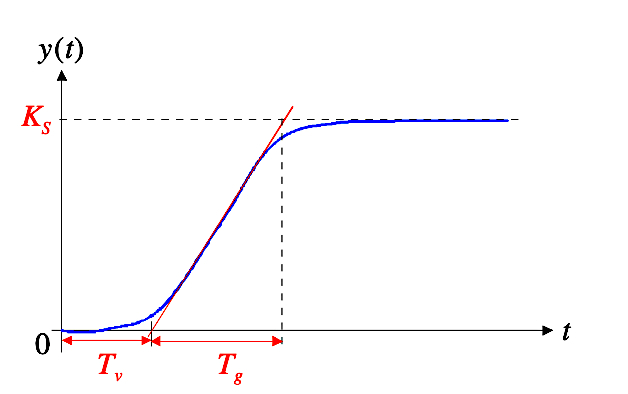
\includegraphics[width=0.8\textwidth]{images/param_zn.jpg}
   \caption[Inflection tangent method Ziegler Nichols]{Inflection tangent method Ziegler Nichols}
   \label{fig:param_zn}
 \end{figure}
The gain $K_{P}$, the delay time $T_{v}$ and the settling time $T_{g}$ can be read from the graph.
The calculation of the controller parameters is performed according to the data in \tablename~\ref{tab:param_zn}. The factor $K_{p}$ from the table equals the term $K_{p}$ in (\ref{eq:pi_contr_2}), while the factor $K_{I}$ is calculated to:
\begin{equation}
    K_{I}  = \frac{K_{P}}{T_{N}}.
 \label{eq:K_I}
\end{equation}
\begin{table}
  \centering
  \begin{tabularx}{0.6\textwidth}{c|c|c|c}
    \toprule
    Controller type & $K_{P}$ &  $T_{N}$ & $T_{D}$   \\
    \midrule
    P-Controller &  $\frac{T_{G}}{K_{S}T_{v}}$ & - & - \\
    & & & \\
    PI-Controller & $0.9\frac{T_{G}}{K_{S}T_{v}}$ & $3.33T_{v}$ & - \\
    & & & \\
    PID-Controller & $0.9\frac{T_{G}}{K_{S}T_{v}}$ & $2T_{v}$ & $0.5T_{v}$ \\
     \bottomrule
  \end{tabularx}
  \caption[Tuning parameters Ziegler Nichols]{Tuning parameters according to Ziegler Nichols}
  \label{tab:param_zn}
\end{table}

\subsubsection{Tuning rules according to Chien Hrones Reswick}
The tuning method accoring to Chien Hrones Reswick is a very similar one to the one by Ziegler Nichols. However, this method provides the ability to adjust the transient response of the control loop. The tuning parameters can either be chosen in a way to probide an over damped behavior or a course providing 20\% overshoot.\cite{Reg_11}
For both options the step response and it's inflection tangent is graphically displayed, as for the Ziegler Nichols approach in \figurename~\ref{fig:param_zn}.
The values for $K_{P}$, $T_{v}$ and $T_{g}$ are read from the plot. The parameter value $K_{I}$ again is calculated following (\ref{eq:K_I}). \tablename~\ref{tab:param_chr} gives the formulas for calculation of $K_{P}$,  $T_{N}$ and $T_{D}$.

\begin{table}
  \centering
  \begin{tabular}{c|ccc|ccc}
    \toprule
     & \multicolumn{3}{c|}{over damped} & \multicolumn{3}{c}{20\% overshoot} \\
    \midrule
    Controller type & $K_{P}$ &  $T_{N}$ & $T_{D}$ & $K_{P}$ &  $T_{N}$ & $T_{D}$ \\
    \midrule
    P-Controller & $0.3\frac{T_{G}}{K_{S}T_{v}}$ & - & - & $0.7\frac{T_{G}}{K_{S}T_{v}}$ & - & - \\
    & & & & & & \\
    PI-Controller & $0.35\frac{T_{G}}{K_{S}T_{v}}$ & $1.2T_{g}$ & - & $0.6\frac{T_{G}}{K_{S}T_{v}}$ & $T_{g}$ & - \\
        & & & & & & \\
    PID-Controller & $0.6\frac{T_{G}}{K_{S}T_{v}}$ & $T_{g}$ & $0.5T_{v}$ & $0.95\frac{T_{G}}{K_{S}T_{v}}$ & $1.35T_{g}$ & $0.47T_{v}$\\
    \bottomrule
\end{tabular}
  \caption[Tuning parameters Chien Hrones Reswick]{Tuning parameters according to Chien Hrones Reswick}
  \label{tab:param_chr}
\end{table}

\section{Iterative Learning Control}
